\chapter{Introducción}

\section{Descripción General}
Se implementará un sistema en chip (SoC) con microprocesador Soft-Core sobre FPGA. El proyecto estará bajo el paradigma de software libre incluyendo
el código RTL del SoC, las herramientas de desarrollo y los Sistema Operativos. Inicialmente se analizarán las diferentes alternativas de
Microprocesadores Soft-Core que permitan su implentación en proyectos SoC Open-Source tales como MinSoC y ORPSoC. El elemento central de
ambos proyectos es el microprocesador soft OpenRisc1200, de capacidades comparables a los microprocesadores soft MicroBlaze de Xilinx y NiOS II de
Altera. Este procesador está soportado por el compilador GCC y permite correr el sistema operativo Linux. El funcionamiento del sistema se comproborá
implementándose sobre un Kit XtremeDSP Starter Platform disponible en el Centro Universitario de Automatización y Robótica UTN-FRC.

\section{Objetivos}
\subsection{Objetivo General}

Implementar un System on Chip OpenSource con Microprocesador Softcore embebido que soporte un Sistema Operativo libre, con la finalidad de entregar
un sistema integral FPGA-SoC-Sistema Operativo completamente funcional y bajo licencia de hardware siguiendo el modelo de Licencia Pública General Menor (LGPL) para el software.


\subsection{Objetivo Específico}
\begin{itemize}
\item Seleccionar, analizar y determinar la factibilidad de implementación de un microprocesador Softcore en FPGA.
% No es seleccionar el SoC tamb 
\item Establecer un System on Chip Open Source donde poder implementar un Softcore.
%o LGPL ???
\item Determinar los Sistemas Operativos con licencia GPL v2 que poseean las prestaciones funcionales adecuadas para su utilización en Sistemas
Embebidos de propósito específico(Por ej.: Sistemas de tiempo real).
\end{itemize}

\section{Motivación} 

Existe un grupo de cores Softcore de código abierto que no están limitados por la tecnología. Los cores destacados de microprocesadores de 32 bits,
son los procesadores SPARC LEON OpenRISC 1200 , y el core de LatticeMico32. Usar cores de código abierto va unido a una serie de conceptos como:
\begin {itemize}
\item
\textit{Flexibilidad}  Si el código fuente está disponible, los desarrolladores pueden modificar el código de acuerdo a sus necesidades. Además, se
produce un flujo constante de ideas que mejoran la calidad del código.
\item 
\textit{Fiabilidad y seguridad}  Con muchos programadores a la vez escrutando el mismo trabajo, los errores se detectan y corrigen antes, por lo que
el producto resultante es mas fiable y eficaz que el comercial.
\item 
\textit{Rapidez de desarrollo}  Las actualizaciones y ajustes se realizan a través de una comunicación constante vía Internet.
\item 
\textit{Relación con el usuario} El programador se acerca mucho mas a las necesidades reales de su cliente, y puede crear un producto específico para
él.
 \end {itemize}
 
Obtener un Sistema Integral de código abierto en donde se tiene código HDL, assembler y C disponible para adaptarse de acuerdo a los requerimientos
del proyecto, además de la capacidad de migrar de una plataforma a otra logrando menor dependencia entre el código fuente y la plataforma
objetivo. La portabilidad del código abierto nos permite implementarlo sobre un ASICs (Application-specific integrated circuit) o con modificaciones
menores en cualquier FPGA (Field Programmable Gate Array) de Xilinx, Altera, Lattice, etc. Estos tres de los más grandes proveedores de FPGA  %,% Xilinx , Altera y Lattice ,
ofrecen sus propios microcore RISC de 32bits como lo son Nios de  Altera y Microblaze de Xilinx  Son micro cores en donde el código fuente RTL no se
encuera disponible y solo pueden ser implementados en las FPGA del propio fabricante.

Una de principales ventajas de usar plataformas con FPGA, es que son flexibles y pueden adaptarse a diferentes funciones. Los componentes de
hardware ofrecen mucho mayor rendimiento que el software equivalente. Los cuellos de botella de procesamiento del sistema pueden identificarse y
sustituirse por hardware, de manera que se evita la costosa optimización del software.

\section{Importancia del Problema}

En el diseño del sistema embebido se usan diferentes procesos dependiendo del tipo de sistema, el hardware disponible y la organización que
desarrolle el sistema. Una de las actividades principales en un proceso de diseño de software es la elección del hardware y del sistema operativo que
se efectúa antes del desarrollo del software. Ante tal situación, se debe diseñar el software considerando las restricciones impuestas por las
capacidades del hardware.
Los efectos que influyen dichas elecciones comprenden restricciones de temporización sobre el sistema, limitación en la energía disponible,
experiencia del equipo de desarrollo y límites en el costos del sistema entregable.
 
Se está explorando una línea donde se busca dar al diseñador del sistema embebido una solución flexible en la primera etapa de la elección de
plataforma. Donde a través del análisis de diferentes plataformas de desarrollo OpenSource y privativas se pueda elegir la mejor opción para el tipo
de sistema a desarrollar y los requerimientos de procesamiento.
 
Una vez que se ha elegido la plataforma de ejecución para el sistema, se ha diseñado una arquitectura de proceso y se ha determinado una política de
planeación, es necesario comprobar que el sistema cumplirá sus con sus requerimientos.

\section{Modelo de Desarrollo}

El modelo de desarrollo a utilizar es el Modelo en Espiral tipificado por Ian Sommerville\cite{Etiqueta00}% . El modelo en espiral de ingeniería de software,mostrado en la figura 1.1
, fue originalmente propuesto por Boehm en año 1988, en su artículo "A Spiral Model of Software Development and Enhancement". Propuso un
marco del proceso de software dirigido por el riesgo. Aquí, el proceso de software se representa como una es espiral, cada ciclo en la espiral
representa una fase del proceso de software. Por ende, el ciclo más interno puede relacionarse con la factibilidad del sistema, el siguiente ciclo
con la definición de requerimientos, el siguiente ciclo al diseño del sistema, y así sucesivamente. %Aclarar que lo implementamos para implementar
% HW...

\begin{figure}[h!]
 \begin{center}
  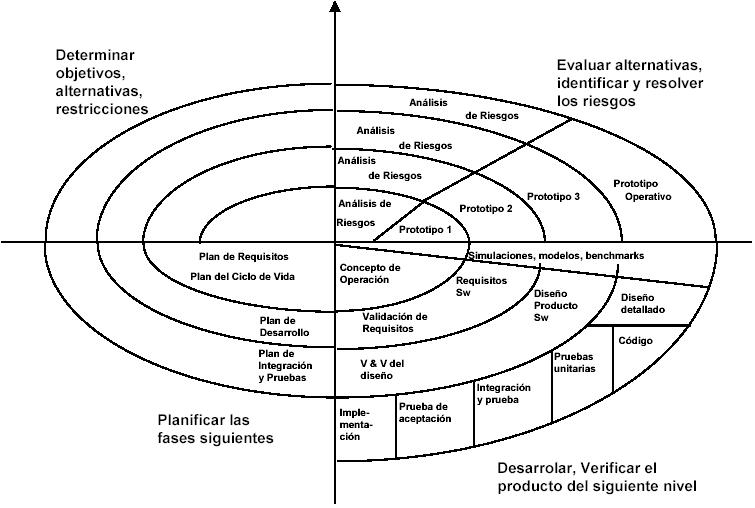
\includegraphics[width=0.5\textwidth,keepaspectratio=true]{./images/ESPIRAL}
  \caption{Etapas del modelo de desarrollo en espiral}
  \label{fig:esquema}
 \end{center}
\end{figure}

Cada ciclo del espiral se divide en 4 sectores:
 
\begin {itemize}
\item 
\textit{Establecimiento de objetivo}  Se definen objetivos específicos para dicha fase del proyecto. Se identifican restricciones en el proceso y el
producto y se traza un plan detallado de gestión. Se identifican los riesgos del proyecto. Dependiendo de estos riegos, se planean estrategias
alternativas que permitan utilizar otros caminos hacia la solución ante sobre la aparición de problemas asociados a estos riesgos.
\item 
\textit{Validación y reducción del riesgo}  En cada uno de los riesgos identificados del proyecto, se realiza un análisis minucioso proponiendo
acciones para reducir dichos riesgos.
\item 
\textit{Desarrollo y validación}  Después de una evaluacion de riesgos, se elige un modelo de desarrollo para el sistema.
\item 
\textit{Planeamiento}  El proyecto se revisa y se toma una decisión sobre si hay que continuar con otro ciclo de la espiral. Si se opta por continuar,
se trazan los planes para la siguente fase del proyecto.
\end {itemize}

Como característica principal de esta metodología es que posee una consideración explícita del riesgo. Informalmente, el riesgo significa
sencillamente que algo puede ir mal. Los riegos originan problemas en el proyecto, como los de confección de agendas y excesos en los costos, por lo
tanto, la disminución de riegos es una actividad sumamente importante en la gestión del proyecto. Un ciclo en la espiral comienza con la elaboración
de objetivos, como el rendimiento y la funcionalidad. Entonces se enumeran formas alternativas de alcanzar estos objetivos y las restricciones
impuestas en cada una de ellas. Cada alternativa se evalúa contra cada objetivo y se identifican las fuentes de riegos del proyecto. El siguiente
paso es resolver estos riesgos mediante actividades de recopilación de información como la de detallar más el análisis, la construcción de prototipos
y la simulación. Una vez que se han evaluado los riesgos se llevará a cabo cierto desarrollo, seguido de una actividad de planificación para la
siguiente fase del proceso.

%El softcore OpenRisc  que se encuentra en el SoC OrpSoc y MinSoc se tiene que implementado en una FPGA  Spartan 3A de Xilinx. Tenemos como fin montar un Linux para validar y verificar el sistema global entregando un sistema funcional bajo licencia libre.
%Actualmente las FPGAs nos birndan la posibilidad de implementar estos proyectos, donde el Hardware y el Software son una misma entidad. Este nuevo enfoque nos permite aprovechar la facilidad de implementar soluciones por Hardware.

\section{Alcance de Estudio}
%En cada etapa ????
Debido al plazo estipulado para el desarrollo del proyecto, el mismo involucra tres etapas: 

\begin {itemize}
\item Especificación y Análisis de requerimientos.
\item Implementación.
\item Testing.
\end {itemize}


\section{Metodología}
%% Primera vez en la facultad???
Considerando que el objetivo planteado es un desarrollo que se realiza por primera vez, se aplicará un desarrollo experimental y de simulación. La
falta de documentación al respecto y al ser un desarrollo de vanguardia son factores que acentúan en esta decisión. Sumado a lo dicho anteriormente,
en el laboratorio donde se desarrolla este proyecto no existen antecedentes de trabajos similares que involucren Microprocesadores Softcore.


%% Esto esta incompleto. 
Se utilizó como metodología en esta implementación el modelo de componentes que define estándares para tal fin, documentación y el
despliegue de componentes.





%%%%% poner en negrita asi \textit{Python} 


